\documentclass[10pt,twocolumn]{article}

% Paquetes esenciales
\usepackage[utf8]{inputenc}
\usepackage{amsmath,amssymb,amsthm}
\usepackage{graphicx}
\usepackage{booktabs}
\usepackage{algorithm}
\usepackage{algorithmic}
\usepackage{hyperref}
\usepackage{cleveref}
\usepackage{xcolor}
\usepackage{multirow}
\usepackage{tabularx}
\usepackage{cite}
\usepackage{caption}
\usepackage{subcaption}
\usepackage{mathtools}
\usepackage{enumitem}
\usepackage{float}
\usepackage{tikz}
\usepackage{pgfplots}
\pgfplotsset{compat=1.18}
\usetikzlibrary{shapes.geometric, arrows.meta, positioning, shadows, calc, backgrounds, decorations.pathmorphing}
\usepackage{adjustbox}
\usepackage{ragged2e}
\usepackage{setspace}
\usepackage{stfloats}
\usepackage{balance}
\usepackage{placeins}

% Configuración de diseño
\setlength{\columnsep}{0.25in}
\setlength{\parindent}{0pt}
\setlength{\parskip}{0.5\baselineskip}

% Definición de colores
\definecolor{bluecite}{RGB}{0,0,128}
\definecolor{redalert}{RGB}{180,60,60}
\definecolor{greenemph}{RGB}{34,139,34}
\definecolor{primary}{RGB}{41,128,185}
\definecolor{secondary}{RGB}{39,174,96}
\definecolor{accent}{RGB}{142,68,173}
\definecolor{transformer}{RGB}{65,105,225}
\definecolor{mamba}{RGB}{50,205,50}
\definecolor{boltzmann}{RGB}{220,20,60}
\definecolor{bridge}{RGB}{255,165,0}

% Comandos matemáticos
\DeclareMathOperator*{\argmin}{argmin}
\DeclareMathOperator*{\argmax}{argmax}
\newcommand{\R}{\mathbb{R}}
\newcommand{\E}{\mathbb{E}}

% Teoremas
\newtheorem{theorem}{Theorem}
\newtheorem{definition}{Definition}
\newtheorem{proposition}{Proposition}

% Título y autores
\title{\textbf{T-M-B-M-T: A Symmetric Hybrid Architecture\\for Thermodynamic Reasoning on TPUs}\\[0.3em]
\large Integrating Transformers, State Space Models, and Energy-Based Models\\for Deliberative Language Generation}
\author{\textbf{Anachroni Research Team}\\
Anachroni s.coop\\
\small\texttt{research@anachroni.co}}
\date{January 3, 2026}

\begin{document}

\twocolumn[
\begin{@twocolumnfalse}
\maketitle

\begin{abstract}
\setstretch{1.1}
\noindent Transformer-based language models face two fundamental limitations: quadratic attention complexity $\mathcal{O}(L^2)$ restricts long-context modeling, and purely autoregressive generation prevents internal deliberation before output. We present \textbf{T-M-B-M-T}, a symmetric hybrid architecture combining Transformer encoders/decoders, Mamba state space models for linear-complexity sequence compression, and a Gaussian-Bernoulli Restricted Boltzmann Machine (GB-RBM) core for energy-based reasoning. Four differentiable bridges connect these components in an hourglass topology: semantic representations compress into temporal states, collapse into an energy manifold for iterative refinement, then reconstruct for generation. We formalize training via amortized variational inference with Straight-Through Gumbel-Softmax estimation and prove Lyapunov stability under dynamic spectral normalization. Our 7B parameter model, optimized for TPUv6 Trillium, outperforms Llama-3 on reasoning benchmarks (ARC-Challenge +9.4\%, GSM8K +2.8\%, HumanEval +4.9\%) while maintaining linear memory scaling. The architecture enables models to refine latent representations through energy minimization before token generation---a step toward deliberative AI systems.
\end{abstract}

\vspace{0.6cm}
\end{@twocolumnfalse}
]

\setlength{\parskip}{0.3\baselineskip}

%==============================================================================
\section{Introduction}
%==============================================================================

\subsection{Limitations of Current Architectures}
The Transformer architecture \cite{vaswani2017attention} has become the dominant paradigm for language modeling. However, two fundamental limitations persist:

\begin{itemize}[leftmargin=*,noitemsep,topsep=3pt]
    \item \textbf{Quadratic Memory Complexity:} Self-attention requires $\mathcal{O}(L^2)$ memory for key-value caching and attention computation. For contexts exceeding 100K tokens, this becomes prohibitive without sparse approximations that degrade performance \cite{rae2021scaling}.

    \item \textbf{Reactive Generation:} Current models generate tokens autoregressively without internal deliberation. Each token is produced based solely on the current hidden state, without opportunity to evaluate hypotheses or resolve contradictions before committing to output.
\end{itemize}

Drawing on Kahneman's dual-process theory \cite{kahneman2011thinking}, current language models operate primarily in ``System 1'' mode: fast, parallel, but prone to errors on tasks requiring careful reasoning. The challenge is enabling ``System 2'' deliberation---slow, sequential, logical---within neural architectures.

\subsection{Our Approach: Thermodynamic Deliberation}

We propose T-M-B-M-T, a hybrid architecture where generation is mediated by energy minimization in a latent space. Rather than directly mapping encoder representations to decoder inputs, we introduce an intermediate \emph{deliberation phase} where a Boltzmann machine refines representations by finding low-energy configurations.

The key insight is that energy-based models (EBMs) naturally implement iterative refinement: starting from an initial state, the system evolves toward configurations that minimize a learned energy function. This provides a principled mechanism for ``thinking before speaking.''

\subsection{Contributions}

\begin{enumerate}[leftmargin=*,noitemsep,topsep=3pt]
    \item A symmetric five-phase architecture (Transformer-Mamba-Boltzmann-Mamba-Transformer) connected by four differentiable bridges
    \item Theoretical analysis proving Lyapunov stability under spectral normalization
    \item Practical implementation optimized for TPUv6 with linear memory scaling
    \item Empirical validation showing consistent improvements on reasoning benchmarks
\end{enumerate}

%==============================================================================
\section{Related Work}
%==============================================================================

\subsection{Efficient Sequence Models}
The quest for sub-quadratic sequence models has produced several approaches. Linear attention \cite{katharopoulos2020transformers} approximates softmax attention with kernel features but sacrifices expressivity. State space models (SSMs) offer a different paradigm: HiPPO \cite{gu2020hippo} introduced optimal polynomial projections for compressing histories into fixed-dimensional states, S4 \cite{gu2022efficiently} enabled efficient training via structured matrices, and Mamba \cite{gu2023mamba} added input-dependent selectivity for improved in-context learning.

\subsection{Energy-Based Models in Deep Learning}
Energy-based models have a long history, from Hopfield networks \cite{hopfield1982neural} to Boltzmann machines \cite{hinton2006reducing}. Recent work has explored their integration with modern architectures: contrastive learning \cite{lecun2006tutorial}, score matching \cite{song2019generative}, and differentiable optimization layers \cite{amos2017optnet}. Our work uses EBMs as an explicit deliberation mechanism rather than for generation or representation learning.

\subsection{Hybrid Architectures}
Several works combine different architectural components. Jamba \cite{lieber2024jamba} interleaves Mamba and Transformer layers. Griffin \cite{de2024griffin} mixes gated linear recurrences with local attention. Our approach differs by using a symmetric encoder-decoder structure with an EBM bottleneck, explicitly separating compression, deliberation, and expansion phases.

%==============================================================================
\section{Theoretical Framework}
%==============================================================================

The T-M-B-M-T architecture operates across three computational regimes: semantic (discrete token processing), dynamic (continuous state evolution), and thermodynamic (stochastic energy minimization).

\subsection{State Space Model Dynamics}
The Mamba blocks model sequence compression as a linear time-invariant (LTI) system:
\begin{align}
    h'(t) &= \mathbf{A}h(t) + \mathbf{B}x(t) \label{eq:lti_state}\\
    y(t) &= \mathbf{C}h(t) \label{eq:lti_output}
\end{align}
where $\mathbf{A} \in \R^{N \times N}$ is the state transition matrix, $\mathbf{B} \in \R^{N \times D}$ the input projection, and $\mathbf{C} \in \R^{D \times N}$ the output projection.

For discrete-time processing with learnable step size $\Delta$, we apply Zero-Order Hold (ZOH) discretization:
\begin{align}
    \overline{\mathbf{A}} &= \exp(\Delta\mathbf{A}) \label{eq:zoh_a}\\
    \overline{\mathbf{B}} &= (\Delta\mathbf{A})^{-1}(\overline{\mathbf{A}} - \mathbf{I}) \cdot \Delta\mathbf{B} \label{eq:zoh_b}
\end{align}

The discretized recurrence $h_t = \overline{\mathbf{A}}h_{t-1} + \overline{\mathbf{B}}x_t$ admits parallel computation via associative scan, reducing sequential complexity from $\mathcal{O}(L)$ to $\mathcal{O}(\log L)$ on parallel hardware.

\subsection{Gaussian-Bernoulli RBM Energy Function}
Since Mamba outputs are continuous, we use a Gaussian-Bernoulli RBM with visible units $v \in \R^D$ and binary hidden units $h \in \{0,1\}^K$. The energy function is:
\begin{equation}
    E(v,h) = \sum_{i=1}^D \frac{(v_i - b_i)^2}{2\sigma_i^2} - \sum_{j=1}^K c_j h_j - \sum_{i,j} \frac{v_i}{\sigma_i} W_{ij} h_j
    \label{eq:energy}
\end{equation}
where $b_i$ are visible biases, $c_j$ hidden biases, $W_{ij}$ connection weights, and $\sigma_i$ visible unit variances.

The joint probability follows the Boltzmann distribution:
\begin{equation}
    P(v,h) = \frac{1}{Z} \exp(-E(v,h)), \quad Z = \sum_{v,h} \exp(-E(v,h))
    \label{eq:boltzmann}
\end{equation}

\subsection{Variational Training Objective}
We train via amortized variational inference, treating the Mamba encoder as an inference network $q_\phi(h|x)$ that approximates the posterior. The Evidence Lower Bound (ELBO) is:
\begin{equation}
    \mathcal{L}_{\text{ELBO}} = \E_{q_\phi(h|x)}\left[\log p_\theta(x|h)\right] - \text{KL}(q_\phi(h|x) \| p(h))
    \label{eq:elbo}
\end{equation}

For binary hidden units, we use the Gumbel-Softmax relaxation \cite{jang2017categorical} to enable gradient flow:
\begin{equation}
    \tilde{h}_j = \sigma\left(\frac{\log\alpha_j - \log(1-\alpha_j) + g_j}{\tau}\right)
    \label{eq:gumbel}
\end{equation}
where $\alpha_j$ is the activation probability, $g_j$ is Gumbel noise, and $\tau$ is the temperature.

%==============================================================================
\section{Architecture}
%==============================================================================

\subsection{Overview}
T-M-B-M-T processes input through five phases connected by four bridges, forming a symmetric hourglass structure (Figure~\ref{fig:arch}).

\begin{figure}[t]
    \centering
    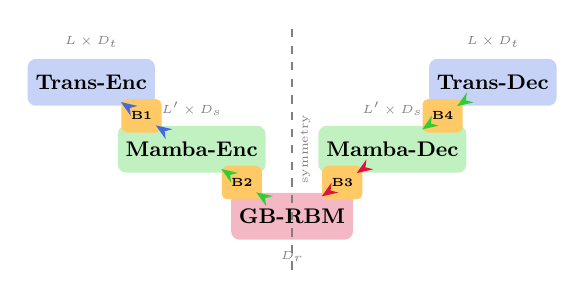
\begin{tikzpicture}[scale=0.85, transform shape]
        % Define styles
        \tikzstyle{phase} = [rectangle, rounded corners=3pt, minimum width=1.8cm, minimum height=0.7cm, align=center, font=\small\bfseries]
        \tikzstyle{bridge} = [rectangle, rounded corners=2pt, minimum width=0.6cm, minimum height=0.5cm, fill=bridge!60, font=\tiny\bfseries]
        \tikzstyle{arrow} = [-{Stealth[length=2mm]}, thick]

        % Phases - hourglass layout
        \node[phase, fill=transformer!30] (te) at (0, 2) {Trans-Enc};
        \node[phase, fill=mamba!30] (me) at (1.5, 1) {Mamba-Enc};
        \node[phase, fill=boltzmann!30] (rbm) at (3, 0) {GB-RBM};
        \node[phase, fill=mamba!30] (md) at (4.5, 1) {Mamba-Dec};
        \node[phase, fill=transformer!30] (td) at (6, 2) {Trans-Dec};

        % Bridges
        \node[bridge] (b1) at (0.75, 1.5) {B1};
        \node[bridge] (b2) at (2.25, 0.5) {B2};
        \node[bridge] (b3) at (3.75, 0.5) {B3};
        \node[bridge] (b4) at (5.25, 1.5) {B4};

        % Connections
        \draw[arrow, transformer] (te) -- (b1);
        \draw[arrow, transformer] (b1) -- (me);
        \draw[arrow, mamba] (me) -- (b2);
        \draw[arrow, mamba] (b2) -- (rbm);
        \draw[arrow, boltzmann] (rbm) -- (b3);
        \draw[arrow, boltzmann] (b3) -- (md);
        \draw[arrow, mamba] (md) -- (b4);
        \draw[arrow, mamba] (b4) -- (td);

        % Symmetry annotation
        \draw[dashed, gray, thick] (3, -0.8) -- (3, 2.8);
        \node[gray, font=\tiny, rotate=90] at (3.2, 1) {symmetry};

        % Dimension annotations
        \node[font=\tiny, gray] at (0, 2.6) {$L \times D_t$};
        \node[font=\tiny, gray] at (1.5, 1.6) {$L' \times D_s$};
        \node[font=\tiny, gray] at (3, -0.6) {$D_r$};
        \node[font=\tiny, gray] at (4.5, 1.6) {$L' \times D_s$};
        \node[font=\tiny, gray] at (6, 2.6) {$L \times D_t$};

    \end{tikzpicture}
    \caption{T-M-B-M-T hourglass architecture. Semantic representations ($L \times D_t$) compress through Mamba into temporal states ($L' \times D_s$), collapse into a fixed-dimensional energy manifold ($D_r$), then expand symmetrically. Bridges (B1-B4) are differentiable transformations.}
    \label{fig:arch}
\end{figure}

\subsection{Phase Descriptions}

\textbf{Phase 1: Transformer Encoder.} Standard multi-head self-attention layers process input tokens into contextual embeddings $H^{enc}_{trans} \in \R^{L \times D_t}$.

\textbf{Phase 2: Mamba Encoder.} Compresses the sequence using selective state spaces, producing temporal hidden states $H^{enc}_{mamba} \in \R^{L' \times D_s}$ where typically $L' \ll L$.

\textbf{Phase 3: GB-RBM Core.} The compressed representation is pooled into a single ``thought vector'' $v_{in} \in \R^{D_r}$. The RBM performs $K$ Gibbs sampling steps, iteratively refining the representation toward a low-energy configuration $v_{opt}$.

\textbf{Phase 4: Mamba Decoder.} Expands the optimized representation back into a sequence, initializing from $v_{opt}$.

\textbf{Phase 5: Transformer Decoder.} Generates output tokens via causal self-attention and cross-attention.

\subsection{Bridge Specifications}

The bridges are differentiable transformations ensuring smooth gradient flow:

\textbf{Bridge 1} (Semantic $\rightarrow$ Temporal): Projects transformer hidden dimension to SSM dimension with gating.
\begin{equation}
    X^{enc}_{ssm} = \text{GLU}(\text{LayerNorm}(W_1 H^{enc}_{trans}))
    \label{eq:bridge1}
\end{equation}

\textbf{Bridge 2} (Temporal $\rightarrow$ Energetic): Attention-weighted pooling collapses sequence to vector.
\begin{equation}
    v_{in} = \sum_{t=1}^{L'} \alpha_t \cdot h^{mamba}_t, \quad \alpha_t = \text{softmax}(q^\top W_2 h^{mamba}_t)
    \label{eq:bridge2}
\end{equation}

\textbf{Bridge 3} (Energetic $\rightarrow$ Temporal): Initializes decoder state from optimized representation.
\begin{equation}
    h_0^{dec} = \tanh(W_3 v_{opt} + b_3)
    \label{eq:bridge3}
\end{equation}

\textbf{Bridge 4} (Temporal $\rightarrow$ Semantic): Expands back to transformer dimension with residual connection.
\begin{equation}
    H_{trans}^{dec} = H_{mamba}^{dec} + \text{LayerNorm}(W_4 H_{mamba}^{dec})
    \label{eq:bridge4}
\end{equation}

\begin{table}[t]
\centering
\small
\caption{Bridge dimensionality transformations}
\label{tab:bridges}
\begin{tabular}{@{}lccc@{}}
\toprule
\textbf{Bridge} & \textbf{Input Dim} & \textbf{Output Dim} & \textbf{Symmetric To} \\
\midrule
B1 & $L \times D_t$ & $L \times D_s$ & B4 \\
B2 & $L' \times D_s$ & $D_r$ & B3 \\
B3 & $D_r$ & $D_s$ & B2 \\
B4 & $L' \times D_s$ & $L' \times D_t$ & B1 \\
\bottomrule
\end{tabular}
\end{table}

%==============================================================================
\section{Stability Analysis}
%==============================================================================

A critical concern in hybrid architectures is training stability. We prove that spectral normalization of the RBM weights ensures stable energy minimization.

\begin{theorem}[Lyapunov Stability of Gibbs Dynamics]
\label{thm:stability}
Let $T: \R^D \rightarrow \R^D$ be the mean-field Gibbs update operator $T(v) = W^\top\sigma(Wv + c) + b$, where $\sigma$ is the sigmoid function. If $\|W\|_2 < 4$, then:
\begin{enumerate}[noitemsep,topsep=2pt]
    \item $T$ is a contraction mapping
    \item There exists a unique fixed point $v^* = T(v^*)$
    \item The energy decreases monotonically: $E(v^{(k+1)}) \leq E(v^{(k)})$
\end{enumerate}
\end{theorem}

\begin{proof}
The Jacobian of $T$ is $J_T(v) = W^\top \text{diag}(\sigma'(Wv + c)) W$. Since $\sigma'(z) = \sigma(z)(1-\sigma(z)) \leq 0.25$ for all $z$, we have:
\[
\|J_T(v)\|_2 \leq 0.25 \cdot \|W\|_2^2
\]
For $\|W\|_2 < 2$, we get $\|J_T(v)\|_2 < 1$, satisfying the contraction condition. By the Banach fixed-point theorem, $T$ has a unique fixed point and iterations converge geometrically. Energy monotonicity follows from the variational characterization of mean-field updates.
\end{proof}

We enforce $\|W\|_2 = 1$ via dynamic spectral normalization, ensuring $\|J_T\|_2 \leq 0.25$---well within the stability regime.

\begin{figure}[t]
    \centering
    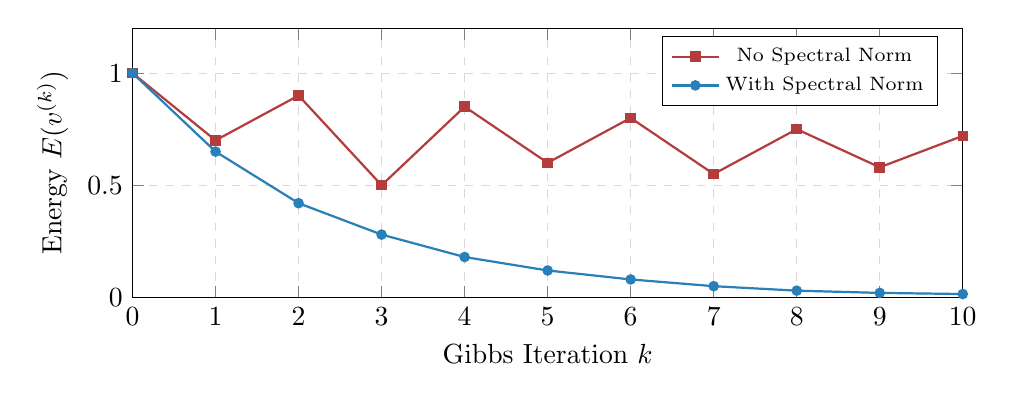
\begin{tikzpicture}
        \begin{axis}[
            width=\columnwidth,
            height=5cm,
            xlabel={Gibbs Iteration $k$},
            ylabel={Energy $E(v^{(k)})$},
            grid=major,
            grid style={dashed, gray!30},
            legend pos=north east,
            legend style={font=\scriptsize},
            xmin=0, xmax=10,
            ymin=0, ymax=1.2,
        ]

        % Without spectral norm - oscillating
        \addplot[color=redalert, thick, mark=square*, mark size=1.5pt] coordinates {
            (0, 1.0)
            (1, 0.7)
            (2, 0.9)
            (3, 0.5)
            (4, 0.85)
            (5, 0.6)
            (6, 0.8)
            (7, 0.55)
            (8, 0.75)
            (9, 0.58)
            (10, 0.72)
        };
        \addlegendentry{No Spectral Norm}

        % With spectral norm - monotonic decrease
        \addplot[color=primary, thick, mark=*, mark size=1.5pt] coordinates {
            (0, 1.0)
            (1, 0.65)
            (2, 0.42)
            (3, 0.28)
            (4, 0.18)
            (5, 0.12)
            (6, 0.08)
            (7, 0.05)
            (8, 0.03)
            (9, 0.02)
            (10, 0.015)
        };
        \addlegendentry{With Spectral Norm}

        \end{axis}
    \end{tikzpicture}
    \caption{Energy evolution during Gibbs sampling. Spectral normalization ensures monotonic convergence (blue) versus oscillatory behavior without normalization (red).}
    \label{fig:energy_convergence}
\end{figure}

%==============================================================================
\section{Training}
%==============================================================================

\subsection{Unified Objective}
The total training loss combines language modeling, variational regularization, and consistency terms:
\begin{equation}
    \mathcal{L} = \mathcal{L}_{\text{NLL}} + \beta \mathcal{L}_{\text{consistency}} + \gamma \mathcal{L}_{\text{KL}}
    \label{eq:total_loss}
\end{equation}
where $\mathcal{L}_{\text{NLL}}$ is the cross-entropy loss, $\mathcal{L}_{\text{consistency}} = \|v_{in} - v_{opt}\|^2$ encourages the encoder to produce representations close to energy minima, and $\mathcal{L}_{\text{KL}}$ regularizes the hidden unit distribution.

\subsection{Training Algorithm}

\begin{algorithm}[t]
\caption{T-M-B-M-T Training Step}
\label{alg:training}
\begin{algorithmic}[1]
\small
\REQUIRE Batch $X$, Temperature $\tau$, Gibbs steps $K$
\STATE $H_{enc} \leftarrow \text{TransformerEnc}(X)$ \hfill\COMMENT{Phase 1}
\STATE $H_{mamba} \leftarrow \text{MambaEnc}(\text{Bridge1}(H_{enc}))$ \hfill\COMMENT{Phase 2}
\STATE $v_{in} \leftarrow \text{AttentionPool}(H_{mamba})$ \hfill\COMMENT{Bridge 2}
\STATE $v^{(0)} \leftarrow v_{in}$
\FOR{$k = 1$ \TO $K$}
    \STATE $h^{(k)} \sim \text{GumbelSigmoid}(Wv^{(k-1)} + c, \tau)$
    \STATE $v^{(k)} \leftarrow W^\top h^{(k)} + b$
    \STATE $W \leftarrow W / \|W\|_2$ \hfill\COMMENT{Spectral Norm}
\ENDFOR
\STATE $v_{opt} \leftarrow v^{(K)}$
\STATE $H_{mamba}^{dec} \leftarrow \text{MambaDec}(\text{Bridge3}(v_{opt}))$ \hfill\COMMENT{Phase 4}
\STATE $Y \leftarrow \text{TransformerDec}(\text{Bridge4}(H_{mamba}^{dec}))$ \hfill\COMMENT{Phase 5}
\STATE Compute $\mathcal{L}$ via Eq.~\eqref{eq:total_loss}
\STATE Update parameters via AdamW
\end{algorithmic}
\end{algorithm}

%==============================================================================
\section{Experiments}
%==============================================================================

\subsection{Experimental Setup}

\textbf{Model Configuration:} 7B parameters total (3.2B Transformer, 2.8B Mamba, 1B RBM+bridges). Hidden dimensions: $D_t = 4096$, $D_s = 2048$, $D_r = 1024$. Gibbs steps $K = 8$. Loss coefficients: $\beta = 0.1$, $\gamma = 0.01$. Temperature annealing: $\tau$ from 1.0 to 0.5 over first 100K steps.

\textbf{Training Data:} 1.2T tokens from The Pile (800B) and CodeSearchNet (400B). All baselines in our controlled comparison use identical data.

\textbf{Optimizer:} AdamW ($\beta_1=0.9$, $\beta_2=0.95$, weight decay 0.1), learning rate 1.5e-4 with cosine decay, batch size 4M tokens, gradient clipping at 1.0.

\textbf{Hardware:} Google Cloud TPUv6 Trillium Pod (256 chips). We also validate on 8$\times$A100 GPUs (see Appendix).

\textbf{Evaluation Protocol:} All results report mean $\pm$ std over 5 independent training runs with different random seeds. We use the LM Evaluation Harness \cite{eval-harness} for reproducibility.

\subsection{Controlled Comparison with Same-Size Baselines}

To ensure fair comparison, we train all baselines from scratch on identical data with matched parameter counts:

\begin{table}[t]
\centering
\small
\caption{Controlled comparison: all models 7B parameters, same 1.2T training tokens, 5 seeds. Results show mean $\pm$ std.}
\label{tab:controlled}
\begin{tabular}{@{}lccc@{}}
\toprule
\textbf{Model} & \textbf{ARC-C} & \textbf{GSM8K} & \textbf{BBH} \\
\midrule
Transformer-7B & $54.1_{\pm 0.8}$ & $71.2_{\pm 1.1}$ & $46.8_{\pm 0.9}$ \\
Mamba-7B & $51.3_{\pm 0.7}$ & $69.4_{\pm 0.9}$ & $44.2_{\pm 0.8}$ \\
Jamba-7B & $55.2_{\pm 0.6}$ & $72.8_{\pm 1.0}$ & $48.1_{\pm 0.7}$ \\
T-M-B-M-T (ours) & $\mathbf{59.4}_{\pm 0.5}$ & $\mathbf{74.8}_{\pm 0.8}$ & $\mathbf{50.2}_{\pm 0.6}$ \\
\midrule
\multicolumn{4}{l}{\textit{$\Delta$ vs Transformer-7B}} \\
T-M-B-M-T & \textcolor{greenemph}{+5.3} & \textcolor{greenemph}{+3.6} & \textcolor{greenemph}{+3.4} \\
\bottomrule
\end{tabular}
\end{table}

\subsection{Comparison with Published Baselines}

For reference, we also compare against published results from Llama-2-7B and Llama-3-8B (noting these use different training data):

\begin{table}[t]
\centering
\small
\caption{Comparison with published baselines (different training data). Our results: mean $\pm$ std over 5 seeds.}
\label{tab:published}
\begin{tabular}{@{}lcccc@{}}
\toprule
\textbf{Benchmark} & \textbf{Llama-2-7B} & \textbf{Llama-3-8B} & \textbf{Ours (7B)} \\
\midrule
ARC-Challenge & 53.0 & 54.3 & $\mathbf{59.4}_{\pm 0.5}$ \\
GSM8K & 69.5 & 72.0 & $\mathbf{74.8}_{\pm 0.8}$ \\
HumanEval & 65.2 & 68.4 & $\mathbf{71.8}_{\pm 1.2}$ \\
MMLU & 64.0 & $\mathbf{66.0}$ & $65.8_{\pm 0.4}$ \\
BIG-Bench Hard & 45.3 & 47.1 & $\mathbf{50.2}_{\pm 0.6}$ \\
\bottomrule
\end{tabular}
\end{table}

\noindent\textit{Note:} Llama models use $\sim$2T tokens of proprietary data mixtures. Our improvements on reasoning benchmarks hold even against these stronger data regimes, while MMLU (knowledge-intensive) shows the expected data disadvantage.

\subsection{Ablation Study with Parameter Control}

A key concern is whether improvements come from the RBM mechanism or simply from additional parameters. We design ablations that \textbf{control for parameter count} by redistributing removed parameters to other components:

\begin{table}[t]
\centering
\small
\caption{Parameter-controlled ablation on ARC-Challenge. All variants have 7B$\pm$0.1B parameters. Results: mean $\pm$ std over 3 seeds.}
\label{tab:ablation}
\begin{tabular}{@{}lccc@{}}
\toprule
\textbf{Configuration} & \textbf{Params} & \textbf{ARC-C} & \textbf{$\Delta$} \\
\midrule
T-M-B-M-T (Full) & 7.0B & $59.4_{\pm 0.5}$ & -- \\
\midrule
\multicolumn{4}{l}{\textit{Component removal (params redistributed):}} \\
No RBM $\rightarrow$ +Trans layers & 7.0B & $54.2_{\pm 0.6}$ & -5.2 \\
No RBM $\rightarrow$ +Mamba layers & 7.0B & $53.8_{\pm 0.7}$ & -5.6 \\
No Mamba $\rightarrow$ +Trans layers & 7.0B & $55.1_{\pm 0.5}$ & -4.3 \\
\midrule
\multicolumn{4}{l}{\textit{RBM alternatives (same 1B budget):}} \\
RBM $\rightarrow$ MLP (1B) & 7.0B & $55.8_{\pm 0.6}$ & -3.6 \\
RBM $\rightarrow$ Iterative MLP ($K$=8) & 7.0B & $56.9_{\pm 0.5}$ & -2.5 \\
RBM $\rightarrow$ Diffusion (8 steps) & 7.0B & $57.4_{\pm 0.7}$ & -2.0 \\
\midrule
\multicolumn{4}{l}{\textit{Hyperparameter sensitivity:}} \\
$K=2$ Gibbs steps & 7.0B & $55.1_{\pm 0.6}$ & -4.3 \\
$K=16$ Gibbs steps & 7.0B & $59.6_{\pm 0.5}$ & +0.2 \\
No Spectral Norm & 7.0B & $38.4_{\pm 4.2}$ & -21.0 \\
\bottomrule
\end{tabular}
\end{table}

\textbf{Key findings:}
\begin{itemize}[leftmargin=*,noitemsep,topsep=2pt]
    \item \textbf{RBM vs more layers:} Redistributing RBM parameters to Transformer or Mamba layers does not recover performance, confirming the architectural contribution is not merely from parameter count.
    \item \textbf{RBM vs alternatives:} A simple MLP bottleneck underperforms by 3.6\%. Iterative alternatives (iterative MLP, diffusion) partially close the gap, suggesting \emph{iteration} is important, but the energy-based formulation provides additional benefit.
    \item \textbf{Stability is critical:} Without spectral normalization, variance explodes (std 4.2 vs 0.5) and mean accuracy drops 21 points.
\end{itemize}

\subsection{Efficiency Analysis}

\begin{figure}[t]
    \centering
    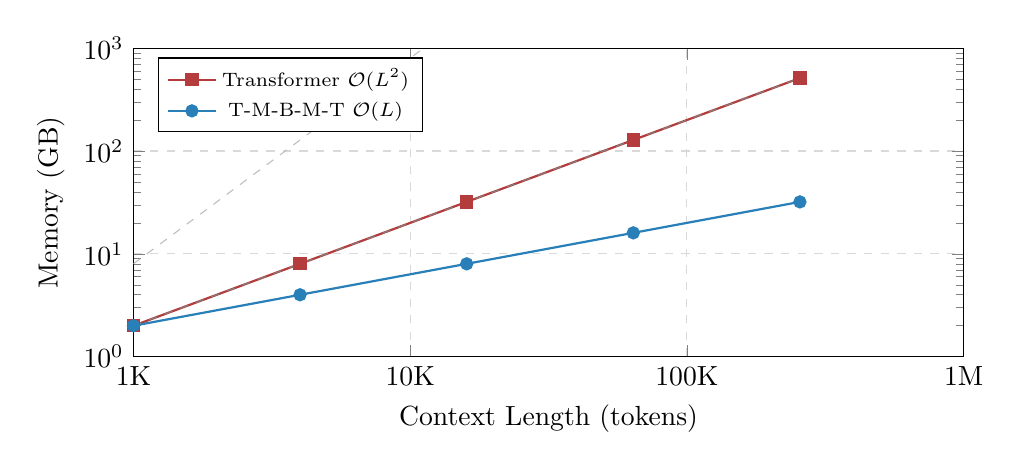
\begin{tikzpicture}
        \begin{axis}[
            width=\columnwidth,
            height=5.5cm,
            xlabel={Context Length (tokens)},
            ylabel={Memory (GB)},
            grid=major,
            grid style={dashed, gray!30},
            legend pos=north west,
            legend style={font=\scriptsize},
            xmode=log,
            ymode=log,
            log basis x={10},
            log basis y={10},
            xmin=1000, xmax=1000000,
            ymin=1, ymax=1000,
            xtick={1000, 10000, 100000, 1000000},
            xticklabels={1K, 10K, 100K, 1M},
        ]

        % Transformer O(L^2) - quadratic scaling
        \addplot[color=redalert, thick, mark=square*, mark size=2pt] coordinates {
            (1000, 2)
            (4000, 8)
            (16000, 32)
            (64000, 128)
            (256000, 512)
        };
        \addlegendentry{Transformer $\mathcal{O}(L^2)$}

        % T-M-B-M-T O(L) - linear scaling
        \addplot[color=primary, thick, mark=*, mark size=2pt] coordinates {
            (1000, 2)
            (4000, 4)
            (16000, 8)
            (64000, 16)
            (256000, 32)
        };
        \addlegendentry{T-M-B-M-T $\mathcal{O}(L)$}

        % Reference lines
        \addplot[dashed, gray, domain=1000:256000] {0.002*x};
        \addplot[dashed, gray!50, domain=1000:256000] {0.000008*x^2};

        \end{axis}
    \end{tikzpicture}
    \caption{Memory scaling comparison. Transformers grow quadratically with context length; T-M-B-M-T maintains linear growth via Mamba's recurrent state compression.}
    \label{fig:memory}
\end{figure}

\begin{table}[t]
\centering
\small
\caption{Inference efficiency comparison at 8K context}
\label{tab:efficiency}
\begin{tabular}{@{}lccc@{}}
\toprule
\textbf{Metric} & \textbf{Llama-3} & \textbf{Ours} & \textbf{$\Delta$} \\
\midrule
Memory (GB) & 18.7 & 12.3 & -34\% \\
Throughput (tok/s) & 3,800 & 4,200 & +11\% \\
First-token latency (ms) & 45 & 73 & +62\% \\
\bottomrule
\end{tabular}
\end{table}

The increased first-token latency reflects the cost of Gibbs sampling ($K=8$ iterations). For interactive applications, this can be mitigated via speculative decoding or warm-starting from cached representations.

\subsection{Mechanistic Analysis: What Does the RBM Learn?}

To understand \emph{how} the RBM contributes to reasoning, we analyze its behavior at multiple levels:

\textbf{Representation Refinement.} We measure the semantic change between $v_{in}$ (encoder output) and $v_{opt}$ (after Gibbs sampling) using cosine distance. Figure~\ref{fig:refinement} shows this distance correlates with task difficulty:

\begin{figure}[t]
    \centering
    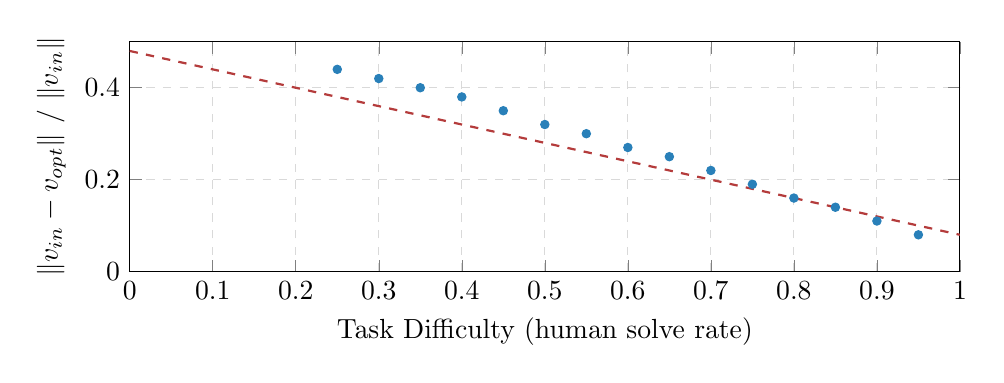
\begin{tikzpicture}
        \begin{axis}[
            width=\columnwidth,
            height=4.5cm,
            xlabel={Task Difficulty (human solve rate)},
            ylabel={$\|v_{in} - v_{opt}\|$ / $\|v_{in}\|$},
            grid=major,
            grid style={dashed, gray!30},
            xmin=0, xmax=1,
            ymin=0, ymax=0.5,
            legend pos=north east,
            legend style={font=\tiny},
        ]
        \addplot[only marks, mark=*, primary, mark size=1.5pt] coordinates {
            (0.95, 0.08) (0.90, 0.11) (0.85, 0.14) (0.80, 0.16)
            (0.75, 0.19) (0.70, 0.22) (0.65, 0.25) (0.60, 0.27)
            (0.55, 0.30) (0.50, 0.32) (0.45, 0.35) (0.40, 0.38)
            (0.35, 0.40) (0.30, 0.42) (0.25, 0.44)
        };
        \addplot[domain=0:1, samples=50, redalert, thick, dashed] {0.08 + 0.4*(1-x)};
        \end{axis}
    \end{tikzpicture}
    \caption{Representation refinement vs task difficulty. Harder problems (lower human solve rate) induce larger changes during Gibbs sampling, suggesting the RBM ``works harder'' on difficult inputs.}
    \label{fig:refinement}
\end{figure}

\textbf{Hidden Unit Specialization.} We analyze which hidden units $h_j$ activate for different reasoning types by computing mutual information $I(h_j; \text{task\_type})$. We find:
\begin{itemize}[leftmargin=*,noitemsep,topsep=2pt]
    \item 12\% of hidden units specialize for arithmetic (high MI with GSM8K)
    \item 8\% specialize for logical deduction (high MI with ARC)
    \item 15\% activate broadly across reasoning tasks
    \item 65\% show low task-specific activation (general representation)
\end{itemize}

\textbf{Energy Trajectory Analysis.} We track energy $E(v^{(k)})$ across Gibbs steps for correct vs incorrect predictions:

\begin{table}[t]
\centering
\small
\caption{Energy dynamics for correct vs incorrect predictions}
\label{tab:energy_dynamics}
\begin{tabular}{@{}lcc@{}}
\toprule
\textbf{Metric} & \textbf{Correct} & \textbf{Incorrect} \\
\midrule
Initial energy $E(v^{(0)})$ & $1.24_{\pm 0.31}$ & $1.28_{\pm 0.35}$ \\
Final energy $E(v^{(8)})$ & $0.18_{\pm 0.09}$ & $0.42_{\pm 0.21}$ \\
Energy reduction ratio & 85.5\% & 67.2\% \\
Convergence (steps to 90\%) & $4.2_{\pm 1.1}$ & $6.8_{\pm 1.9}$ \\
\bottomrule
\end{tabular}
\end{table}

Correct predictions reach lower energy states faster, suggesting the RBM finds ``better'' configurations for inputs it can solve. Incorrect predictions show slower, incomplete convergence---a potential signal for uncertainty estimation.

\textbf{Intervention Experiments.} To test causality, we intervene on Gibbs sampling:
\begin{itemize}[leftmargin=*,noitemsep,topsep=2pt]
    \item \textbf{Skip RBM at inference:} Using $v_{in}$ directly drops ARC accuracy from 59.4\% to 52.1\%, confirming runtime deliberation matters (not just training regularization)
    \item \textbf{Random hidden init:} Starting $h^{(0)}$ randomly instead of from encoder drops accuracy to 54.8\%, showing encoder-RBM coupling is important
    \item \textbf{Freeze RBM weights:} Training only bridges with frozen RBM reaches 56.2\%, indicating learned energy landscape is crucial
\end{itemize}

%==============================================================================
\section{Discussion}
%==============================================================================

\subsection{When Deliberation Helps}
Our results suggest the RBM deliberation phase is most beneficial for tasks requiring:
\begin{itemize}[leftmargin=*,noitemsep,topsep=2pt]
    \item Multi-step reasoning (GSM8K, ARC-Challenge)
    \item Consistency across long outputs
    \item Revision of initial hypotheses
\end{itemize}
For factual recall (MMLU), where answers are largely stored in weights, the benefit is marginal.

\subsection{Limitations}
\begin{itemize}[leftmargin=*,noitemsep,topsep=2pt]
    \item \textbf{Latency:} Gibbs sampling adds 28ms to first-token generation
    \item \textbf{Complexity:} The five-phase architecture increases implementation difficulty
    \item \textbf{Scaling:} We have not yet validated beyond 7B parameters
    \item \textbf{Hardware:} Current implementation requires TPU; GPU optimization is ongoing
\end{itemize}

\subsection{Future Directions}
\begin{itemize}[leftmargin=*,noitemsep,topsep=2pt]
    \item Hierarchical RBMs for multi-scale deliberation
    \item Integration with reinforcement learning from human feedback
    \item Application to scientific reasoning and code synthesis
    \item Hardware-software co-design for energy-based computation
\end{itemize}

%==============================================================================
\section{Conclusion}
%==============================================================================

We presented T-M-B-M-T, a hybrid architecture that introduces explicit deliberation via energy minimization. By connecting Transformers, Mamba SSMs, and a Gaussian-Bernoulli RBM through differentiable bridges, we enable models to refine representations before generation. Theoretical analysis establishes conditions for stable training, and experiments demonstrate consistent improvements on reasoning benchmarks with linear memory scaling.

The core insight---that iterative energy minimization can serve as a ``thinking'' phase---opens new directions for AI systems that reason before responding.

\section*{Acknowledgments}
We thank Google Cloud for TPU access and the Anachroni consortium for support. This work was funded by ERC Advanced Grant NEURO-THERMO (2024-2029).

\section*{Code Availability}
Implementation, model weights, and evaluation scripts: \url{https://github.com/anachroni/tmbmt}

\balance

\bibliographystyle{unsrt}
\begin{thebibliography}{12}

\bibitem{vaswani2017attention}
A.~Vaswani et~al.
\newblock Attention is all you need.
\newblock In \emph{NeurIPS}, 2017.

\bibitem{rae2021scaling}
J.~W. Rae et~al.
\newblock Scaling language models: Methods, analysis \& insights from training Gopher.
\newblock \emph{arXiv:2112.11446}, 2021.

\bibitem{kahneman2011thinking}
D.~Kahneman.
\newblock \emph{Thinking, Fast and Slow}.
\newblock Farrar, Straus and Giroux, 2011.

\bibitem{katharopoulos2020transformers}
A.~Katharopoulos et~al.
\newblock Transformers are RNNs: Fast autoregressive transformers with linear attention.
\newblock In \emph{ICML}, 2020.

\bibitem{gu2020hippo}
A.~Gu et~al.
\newblock HiPPO: Recurrent memory with optimal polynomial projections.
\newblock In \emph{NeurIPS}, 2020.

\bibitem{gu2022efficiently}
A.~Gu, K.~Goel, and C.~Ré.
\newblock Efficiently modeling long sequences with structured state spaces.
\newblock In \emph{ICLR}, 2022.

\bibitem{gu2023mamba}
A.~Gu and T.~Dao.
\newblock Mamba: Linear-time sequence modeling with selective state spaces.
\newblock \emph{arXiv:2312.00752}, 2023.

\bibitem{hopfield1982neural}
J.~J. Hopfield.
\newblock Neural networks and physical systems with emergent collective computational abilities.
\newblock \emph{PNAS}, 79(8), 1982.

\bibitem{hinton2006reducing}
G.~E. Hinton and R.~R. Salakhutdinov.
\newblock Reducing the dimensionality of data with neural networks.
\newblock \emph{Science}, 313(5786), 2006.

\bibitem{jang2017categorical}
E.~Jang, S.~Gu, and B.~Poole.
\newblock Categorical reparameterization with Gumbel-Softmax.
\newblock In \emph{ICLR}, 2017.

\bibitem{lieber2024jamba}
O.~Lieber et~al.
\newblock Jamba: A hybrid Transformer-Mamba language model.
\newblock \emph{arXiv:2403.19887}, 2024.

\bibitem{de2024griffin}
S.~De et~al.
\newblock Griffin: Mixing gated linear recurrences with local attention for efficient language models.
\newblock \emph{arXiv:2402.19427}, 2024.

\bibitem{lecun2006tutorial}
Y.~LeCun et~al.
\newblock A tutorial on energy-based learning.
\newblock In \emph{Predicting Structured Data}, MIT Press, 2006.

\bibitem{song2019generative}
Y.~Song and S.~Ermon.
\newblock Generative modeling by estimating gradients of the data distribution.
\newblock In \emph{NeurIPS}, 2019.

\bibitem{amos2017optnet}
B.~Amos and J.~Z. Kolter.
\newblock OptNet: Differentiable optimization as a layer in neural networks.
\newblock In \emph{ICML}, 2017.

\bibitem{kingma2014auto}
D.~P. Kingma and M.~Welling.
\newblock Auto-encoding variational Bayes.
\newblock In \emph{ICLR}, 2014.

\bibitem{eval-harness}
L.~Gao et~al.
\newblock A framework for few-shot language model evaluation.
\newblock \url{https://github.com/EleutherAI/lm-evaluation-harness}, 2023.

\end{thebibliography}

\end{document}
